\question{Функция Гамильтона. Канонические уравнения Гамильтона. Примеры
применения уравнений Гамильтона.}

Составим полный дифференциал функции Лагранжа как функции обобщенных координат,
скоростей и времени:
\( \ds dL = \sum_{i=1}^s \pder{L}{q_i}\,dq_i + \sum_{i=1}^s \pder{L}{\dot{q}_i}
\,d\dot{q}_i + \pder{L}{t}\,dt \).

Учтем, что \( \ds \pder{L}{\dot{q}_i} = p_i \), а \( \ds \pder{L}{q_i} =
\dot{p}_i \), тогда дифференциал запишется в виде:
\[
    dL = \sum_{i=1}^s \dot{p}_i\,dq_i + \sum_{i=1}^s p_i\d\dot{q}_i +
    \pder{L}{t}dt.
\]
Запишем второе слагаемое в виде:
\[
    \sum_{i=1}^s p_i\d\dot{q}_i = \sum_{i=1}^s d(p_i\dot{q}_i) - \sum_{i=1}^s
    \dot{q}_i\,dp_i = d\left(\sum_{i=1}^s p_i\dot{q}_i\right) - \sum_{i=1}^s
    \dot{q}_i\,dp_i,
\]
тогда \( \ds dL = \sum_{i=1}^s \dot{p}_i\,dq_i + d\left(\sum_{i=1}^s
p_i\dot{q}_i\right) - \sum_{i=1}^s\dot{q}_i\,dp_i + \pder{L}{t}dt \).
Следовательно, перенося полный дифференциал в левую сторону и изменяя знаки,
получаем:
\[
    d\left(\sum_{i=1}^s p_i\dot{q}_i - L\right) = \sum_{i=1}^s\dot{q}_i\,dp_i -
    \sum_{i=1}^s \dot{p}_i\,dq_i - \pder{L}{t}dt.
\]
Введем функцию \( H \), как функцию обобщенных координат, обобщенных импульсов и времени:
\( \ds H(q, p, t) = \sum_{i=1}^s p_i\dot{q}_i - L \), которая носит название
функции Гамильтона. Подставляя функцию Гамильтона в ДУ, получим: \( \ds dH =
\sum_{i=1}^s\dot{q}_i\,dp_i - \sum_{i=1}^s \dot{p}_i\,dq_i - \pder{L}{t}dt \),
откуда получаем канонические уравнения Гамильтона:
\[
    \dot{q}_i = \pder{H}{p_i}, \quad \dot{p}_i = -\pder{H}{q_i}, \quad
    \pder{L}{t} = -\pder{H}{t}.
\]

\subquestion{Пример применения уравнения Гамильтона(в поле силы тяжести)}
\begin{minipage}{.4\textwidth}
    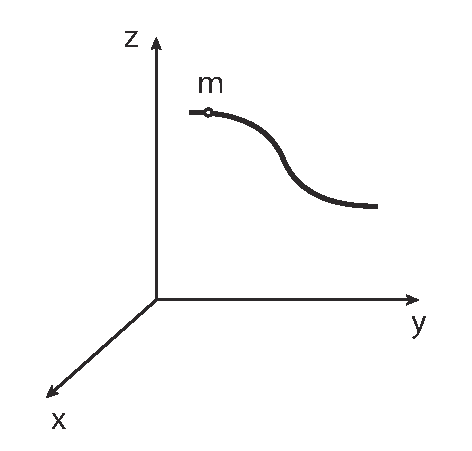
\includegraphics[width=\textwidth]{17_01}
\end{minipage} \hfill
\begin{minipage}{.55\textwidth}
    \begin{gather*}
        H = \frac{1}{2}(m\dot{x}^2 + m\dot{y}^2 + m\dot{z}^2) + mgz. \\
        p_x = \pder{T}{\dot{x}} = m\dot{x}, \quad \dot{x} = \frac{p_x}{m}, \\
        p_y = \pder{T}{\dot{y}} = m\dot{y}, \quad \dot{y} = \frac{p_y}{m}, \\
        p_z = \pder{T}{\dot{z}} = m\dot{z}, \quad \dot{z} = \frac{p_z}{m}. \\
        H = \frac{1}{2}\left( \frac{p_x^2}{m} + \frac{p_y^2}{m} +
        \frac{p_z^2}{m} \right) + mgz,
    \end{gather*}
    следовательно, \( p_x = 0,\ p_y = 0,\ p_z = -mg \).
\end{minipage}

\newpage
